\documentclass[aspectratio=169]{beamer}

\usepackage[utf8]{inputenc}
\usepackage{array}
\usepackage{booktabs}
\usepackage{bold-extra}
\usepackage{graphics}
\usepackage{hyperref}
\hypersetup{%
  colorlinks=true,
  linkcolor=blue,
  filecolor=blue,
  urlcolor=cyan,
}
\usepackage{listings}
\usepackage{multicol}
\usepackage{multirow}
\usepackage[absolute,overlay]{textpos}
\usepackage{setspace}
\usepackage{verbatim}
\usepackage{fancyvrb} % for verbatim centering
\usepackage{tikz}

\usetheme{Warsaw}
\usecolortheme{beaver}
\definecolor{clOrange}{HTML}{E76600}
\definecolor{clAlmostWhite}{HTML}{FEFFD9}
\definecolor{clGreen}{HTML}{007F00}
\definecolor{clFlag}{HTML}{D33682}
\definecolor{clFlagOpt}{HTML}{CB4B16}
\definecolor{clRedFlag}{HTML}{DC322F}
\definecolor{clViolet}{HTML}{4c0070}
\definecolor{clGray}{HTML}{888888}

\definecolor{clCodeBlue}{rgb}{0.0, 0.18, 0.38}
\definecolor{clCodeGreen}{rgb}{0.0, 0.27, 0.15}
\definecolor{clCodeRed}{rgb}{0.63, 0.0, 0.0}


\setbeamertemplate{navigation symbols}{}
\setbeamercolor{title}{fg=black}
\setbeamercolor{author}{fg=clAlmostWhite}
\setbeamercolor{date}{fg=clAlmostWhite}
\setbeamerfont{author}{size=\huge}
\setbeamerfont{date}{size=\Large}

\newcommand{\greenemph}[1]{\textit{\textcolor{clGreen}{#1}}}
\newcommand{\cpp}[1]{\texttt{\textbf{\textcolor{clCodeBlue}{#1}}}}

\newcommand\fontV{\fontsize{5}{5}\selectfont}

\lstset{
  language=C++,
  basicstyle=\ttfamily,
  keywordstyle=\color{clCodeBlue}\ttfamily,
  stringstyle=\color{clCodeGreen}\ttfamily,
  commentstyle=\color{clCodeRed}\ttfamily,
  morecomment=[l][\color{magenta}]{\#}
}

\title[Friends\#23 :: \cpp{IntegerPromotions}]{Integer Promotions in \cpp{C++}}
\author{Adam Graliński}
\date[July'22]{\textbf{\texttt{\color[HTML]{d33682}C++} {\color[HTML]{268bd2}F}{\color[HTML]{2aa198}r}{\color[HTML]{859900}i}%
{\color[HTML]{cb4b16}e}{\color[HTML]{dc322f}n}{\color[HTML]{6c71c4}d}{\color[HTML]{b58900}s}, October 2022}}

\begin{document}

{\usebackgroundtemplate{%
 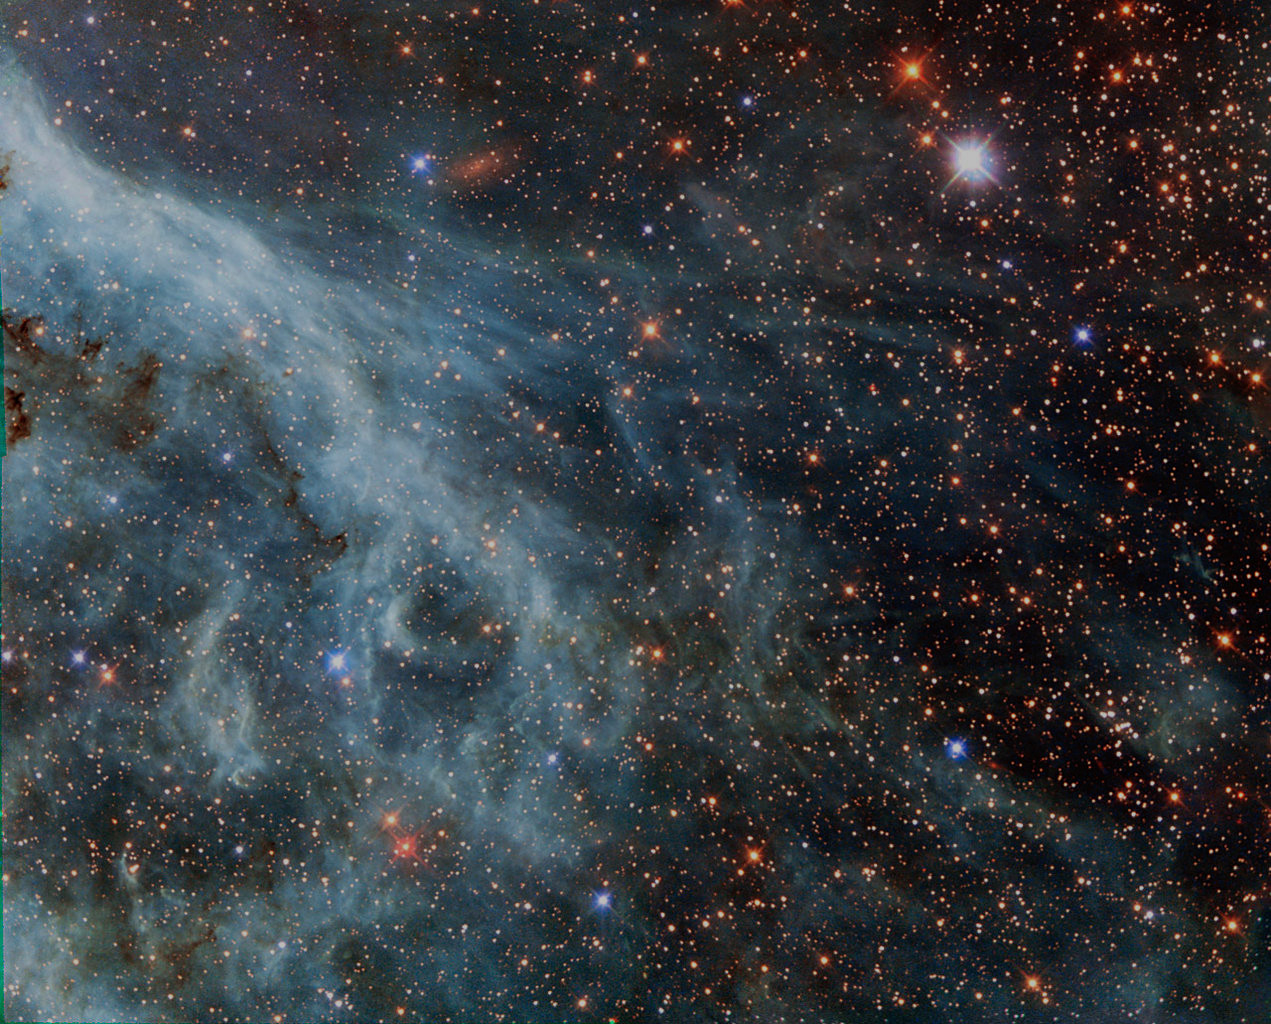
\includegraphics[width=\paperwidth,height=\paperheight]{../common/bg_galaxy.jpg}}
\begin{frame}
\titlepage{}
\end{frame}
}

\begin{frame}[fragile]
\frametitle{Introduction}
\begin{center}
"Use \cpp{int}s unless you need something different.
Then still use something signed, until you \textbf{really} need something
different, at which point --- resort to unsigned" \\
\vspace{12pt}
--- Herb Sutter, Interactive Panel @ Microsoft's Going Native Conference 2013
\end{center}
\end{frame}


\begin{frame}[fragile]
\frametitle{Introduction}
\begin{center}
"Yeah, I was going to say something very similar.
Use \cpp{int}s --- until you have a reason not to. Don't use \cpp{unsigned} unless you're fiddling with bit-patterns,
and never mix \cpp{signed} and \cpp{unsigned}. \\
\vspace{12pt}
--- Bjarne Stroustrup, Interactive Panel @ Microsoft's Going Native Conference 2013 (12:30 in)
\end{center}
\end{frame}


\begin{frame}[fragile]
\frametitle{Pop quiz I}
\begin{columns}[T]
  \begin{column}{0.7\textwidth}<1->
    {\color[HTML]{cb4b16}
    \texttt{\textbf{intro.cpp}}\vspace{-9pt}
    \rule{\linewidth}{2pt}}%
    {\fontsize{8}{6} \lstinputlisting[showstringspaces=false]{code/intro.cpp}}%
    \vspace{-12pt}{\color[HTML]{cb4b16}\rule{\linewidth}{2pt}}%
  \end{column}
  \begin{column}{0.25\textwidth}<2->
    {\color[HTML]{002b36}
    \texttt{\textbf{output}}\vspace{-9pt}
    \rule{\linewidth}{2pt}}%
    {\fontsize{8}{6} \begin{lstlisting}[showstringspaces=false]
-123 < 123: true
-123 < 456: false
    \end{lstlisting}
    }
    \vspace{-12pt}{\color[HTML]{002b36}\rule{\linewidth}{2pt}}%
  \end{column}
\end{columns}
\pause{}
\begin{center}\url{https://godbolt.org/z/ePaWrfexf}\end{center}
\end{frame}


\begin{frame}[fragile]
\frametitle{Pop quiz II}
\begin{columns}[T]
  \begin{column}{0.7\textwidth}<1->
    {\color[HTML]{cb4b16}
    \texttt{\textbf{surprises.cpp}}\vspace{-9pt}
    \rule{\linewidth}{2pt}}%
    {\fontsize{8}{6} \lstinputlisting[showstringspaces=false]{code/surprises.cpp}}%
    \vspace{-12pt}{\color[HTML]{cb4b16}\rule{\linewidth}{2pt}}%
  \end{column}
  \begin{column}{0.25\textwidth}<2->
    {\color[HTML]{002b36}
    \texttt{\textbf{output}}\vspace{-9pt}
    \rule{\linewidth}{2pt}}%
    {\fontsize{8}{6} \begin{lstlisting}[showstringspaces=false]
one == 1,
maxshort == 65535,
sum = maxshort+one = 0
Oh no!
    \end{lstlisting}
    }
    \vspace{-12pt}{\color[HTML]{002b36}\rule{\linewidth}{2pt}}%
  \end{column}
\end{columns}
\pause{}
\begin{center}\url{https://godbolt.org/z/aKzEsaY8q}\end{center}
\end{frame}


\begin{frame}[fragile]
\frametitle{Why?}
\begin{columns}[T]
  \begin{column}{0.7\textwidth}<1->
    \vspace*{-30pt}\
    
\includegraphics[width=0.3\textwidth]{pictures/why1.png}\
    
\includegraphics[width=0.3\textwidth]{pictures/why3.png}\
    
\includegraphics[width=0.3\textwidth]{pictures/why2.png}\
  \end{column}
  \begin{column}{0.35\textwidth}
    \begin{itemize}
      \item{} undefined behavior?
      \item{} cosmic rays?
      \item{} ghost in the machine?
    \end{itemize}
  \end{column}
\end{columns}
\pause{}
\vspace{24pt}
\begin{center}
No, this is \greenemph{well defined behavior}.\\
Both caused by \emph{implicit promotion rules for numeric data types}.
\end{center}
\end{frame}


\begin{frame}[fragile]
\frametitle{cppreference sources}
\begin{center}
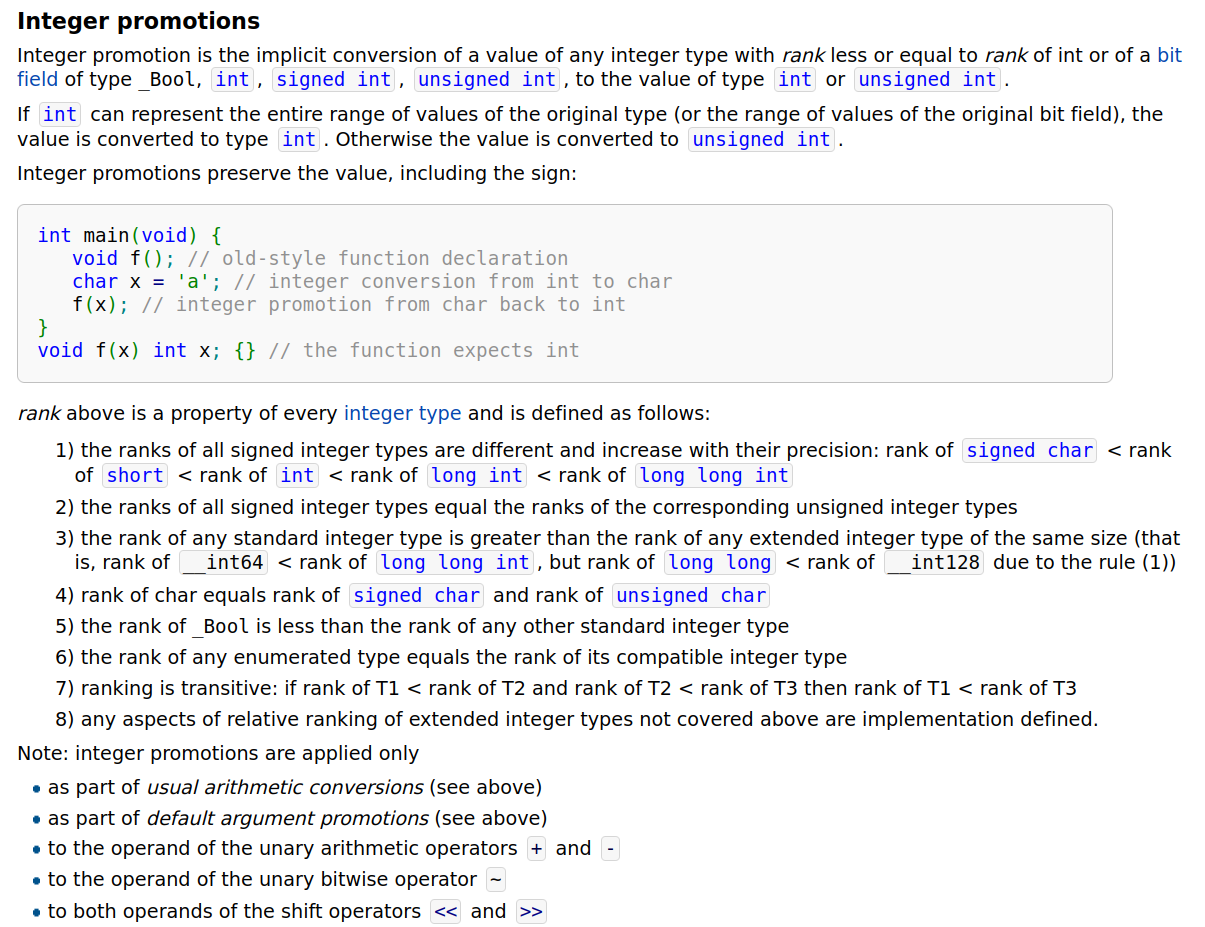
\includegraphics[width=0.6\textwidth]{pictures/cppreference-integer-promotions.png}
\vspace*{12pt}
{\footnotesize \url{https://en.cppreference.com/w/cpp/language/implicit\_conversion#Numeric\_promotions}}
\end{center}
\end{frame}

\begin{frame}[fragile]
\frametitle{Pop quiz I --- explanation}
\begin{columns}[T]
  \begin{column}{0.7\textwidth}<1->
    {\color[HTML]{cb4b16}
    \texttt{\textbf{intro-explained.cpp}}\vspace{-9pt}
    \rule{\linewidth}{2pt}}%
    {\fontsize{4}{4} \lstinputlisting[showstringspaces=false]{code/intro-explained-fragment.cpp}}%
    \vspace{-12pt}{\color[HTML]{cb4b16}\rule{\linewidth}{2pt}}%
  \end{column}
  \begin{column}{0.25\textwidth}<2->
    {\color[HTML]{002b36}
    \texttt{\textbf{output}}\vspace{-9pt}
    \rule{\linewidth}{2pt}}%
    {\fontsize{8}{6} \begin{lstlisting}[showstringspaces=false]
-123 < 123: true
-123 < 456: false
-123(long) is
18446744073709551493
 (unsigned long)
    \end{lstlisting}
    }
    \vspace{-12pt}{\color[HTML]{002b36}\rule{\linewidth}{2pt}}%
  \end{column}
\end{columns}
\pause{}
\begin{center}\url{https://godbolt.org/z/1efG9WP1n}\end{center}
\end{frame}


\begin{frame}[fragile]
\frametitle{Pop quiz II --- explanation}
\begin{columns}[T]
  \begin{column}{0.7\textwidth}<1->
    {\color[HTML]{cb4b16}
    \texttt{\textbf{surprises-explained.cpp}}\vspace{-9pt}
    \rule{\linewidth}{2pt}}%
    {\fontsize{8}{6} \lstinputlisting[showstringspaces=false]{code/surprises-explained.cpp}}%
    \vspace{-12pt}{\color[HTML]{cb4b16}\rule{\linewidth}{2pt}}%
  \end{column}
  \begin{column}{0.25\textwidth}<2->
    {\color[HTML]{002b36}
    \texttt{\textbf{output}}\vspace{-9pt}
    \rule{\linewidth}{2pt}}%
    {\fontsize{8}{6} \begin{lstlisting}[showstringspaces=false]
one == 1,
maxshort == 65535,
sum = maxshort+one = 0
Oh no!

Reminder:
sum = maxshort + one
sum is: 0
(maxshort+one) is: 65536
    \end{lstlisting}
    }
    \vspace{-12pt}{\color[HTML]{002b36}\rule{\linewidth}{2pt}}%
  \end{column}
\end{columns}
\pause{}
\begin{center}\url{https://godbolt.org/z/9WraPPM9v}\end{center}
\end{frame}


\begin{frame}
\frametitle{Key takeaways}
{\centering
\begin{itemize}
  \item{} \textbf{\textcolor{clRedFlag}{never} compare signed and unsigned integers!}
  \item{} enable \greenemph{-Wsign-compare} (and \greenemph{-Werror} to force this).
  \item{} remember that small unsigned ints might be promoted.
  \begin{itemize}
    \item{} Especially that they \textbf{are} promoted when using mathematical operators\\
    (e.g. \cpp{operator+()}, \cpp{operator*()}).
  \end{itemize}
  \item{} also, keep in mind that both \cpp{int32\_t} and \cpp{int64\_t}\\
  are valid candidates for integer promotion, too\\
  \vspace*{-3pt}
  \raggedleft{\tiny \textcolor{clGray}{on platforms where int is of size 64-bits and 128-bits, respectively}}\\
  \raggedright-- we may be writing vulnerable code right now, for the future platforms.
  \begin{itemize}
    \item{} {\tiny although future compiler writers already know this, and will probably provide mitigations}
  \end{itemize}
  \item{} statically-check, lint, sanitize and fuzz your codebases.
\end{itemize}

\vspace{2ex}
\begin{center}{\Large Thank you!}\end{center}
}
\end{frame}

\end{document}
